% !TeX root = ../analisi_2.tex

\section{Topologia in \texorpdfstring{$\mathbb{R}^n$ ($\mathbb{R}^2$)}{R n (R 2)}}

\subsection{Lo spazio \texorpdfstring{$\mathbb{R}^n$}{R n}}

Sia $\mathbb{R}^2 = \mathbb{R} \times \mathbb{R}$
\[
\mathbb{R}^n = \underbrace{\mathbb{R} \times \dots \times \mathbb{R}}_{n\text{-volte}}
\]
In $\mathbb{R}^2$ (e in $\mathbb{R}^n$) si def. le seguenti ``operazioni'':
\begin{itemize}
    \item[$\oplus$] $v_1, v_2 \in \mathbb{R}^2 \implies v_1 + v_2 = (x_1 + x_2, y_1 + y_2)$, dove $v_1 = (x_1, y_1)$, $v_2 = (x_2, y_2)$
    \item[$\odot$] Sia $\alpha \in \mathbb{R}$, $v \in \mathbb{R}^2$ si def.: $\alpha v = (\alpha x, \alpha y) \in \mathbb{R}^2$ dove $v = (x, y)$
\end{itemize}
$\implies (\mathbb{R}^2, +, \cdot)$ sp. vett. su $\mathbb{R}$.

\pencilnote{Scalari con lettere greche e vettori senza sottolineatura.}

\begin{oss}
Si può def. la diff. $v_1 - v_2 = v_1 + (-v_2)$.
\end{oss}

\subsection{Norma, distanza e prodotto scalare}

\begin{definition}
Sia $v \in \mathbb{R}^2$ ($v = (x, y)$), si chiama \underline{norma} di $v$ (o modulo) la seg. quantità:
\[
\vert v \vert = \sqrt{x^2 + y^2} \qquad \left(\text{in } \mathbb{R}^n \quad \vert v \vert = \sqrt{x_1^2 + \dots + x_n^2}\right)
\]
\end{definition}

\textbf{Proprietà:}
\begin{enumerate}
    \item $\forall v \in \mathbb{R}^2$ si ha $\vert v \vert \ge 0$ e $\vert v \vert = 0 \iff v = 0$
    \item $\vert \alpha v \vert = \vert \alpha \vert \vert v \vert \quad \forall \alpha \in \mathbb{R}, \ \forall v \in \mathbb{R}^2$
    \item $\vert v_1 + v_2 \vert \le \vert v_1 \vert + \vert v_2 \vert \quad \forall v_1, v_2 \in \mathbb{R}^2$ \pencilnote{dis. triang. (in un triangolo la lunghezza di un lato è sempre $\le$ somma degli altri 2 lati)}
\end{enumerate}

\pencilnote{Per le funzioni (serve a Metodi): sia $C([a, b]) = \{ f \text{ cont. su } [a, b] \}$, $\|f\| = \max_{[a, b]} \vert f \vert \ge 0$.}

\begin{definition}
Siano $v_1, v_2 \in \mathbb{R}^2$, si def. \underline{distanza} tra $v_1$ e $v_2$ la seg.:
\[
d(v_1, v_2) = \vert v_1 - v_2 \vert = \sqrt{(x_1 - x_2)^2 + (y_1 - y_2)^2}
\]
dove $v_1 = (x_1, y_1)$, $v_2 = (x_2, y_2)$.
\end{definition}

\begin{oss}
In $\mathbb{R}^2$ (in gen. in $\mathbb{R}^n$) non c'è $\le$.
\end{oss}

\begin{definition}
Siano $v_1, v_2 \in \mathbb{R}^2$ si chiama \underline{prodotto scalare} tra $v_1$ e $v_2$ il seguente:
\[
\langle v_1, v_2 \rangle := x_1 x_2 + y_1 y_2 \in \mathbb{R}
\]
se $v_1 = (x_1, y_1)$, $v_2 = (x_2, y_2)$.
\end{definition}

\textbf{Prop.:} $\forall v_1, v_2, v_3 \in \mathbb{R}^2, \ \forall \alpha \in \mathbb{R}$
\begin{enumerate}
    \item $\langle v_1, v_2 \rangle = \langle v_2, v_1 \rangle$
    \item $\langle v_1 + v_2, v_3 \rangle = \langle v_1, v_3 \rangle + \langle v_2, v_3 \rangle$
    \item $\alpha \langle v_1, v_2 \rangle = \langle \alpha v_1, v_2 \rangle = \langle v_1, \alpha v_2 \rangle$
    \item $\langle v, v \rangle = \vert v \vert^2$
    \item $\vert \langle v_1, v_2 \rangle \vert \le \vert v_1 \vert \vert v_2 \vert$
\end{enumerate}

\subsection{Intorni e classificazione dei punti}

\begin{definition}
Sia $v_0 = (x_0, y_0) \in \mathbb{R}^2$. Si chiama \underline{intorno sferico} di $v_0$ di raggio $\delta > 0$ il seg.:
\[
\begin{aligned}
I_\delta(v_0) &= \{ v \in \mathbb{R}^2, v = (x, y) : \vert v - v_0 \vert < \delta \} = \\
&= \{ (x, y) \in \mathbb{R}^2 : \sqrt{(x - x_0)^2 + (y - y_0)^2} < \delta \} = \\
&= \{ (x, y) \in \mathbb{R}^2 : (x - x_0)^2 + (y - y_0)^2 < \delta^2 \}
\end{aligned}
\]
\pencilnote{(senza ``bordo'')}
\end{definition}

\begin{center}
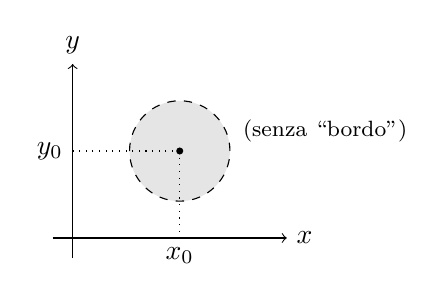
\begin{tikzpicture}[scale=0.85]
    \draw[->] (-0.3,0) -- (3.2,0) node[right] {$x$};
    \draw[->] (0,-0.3) -- (0,2.6) node[above] {$y$};
    \fill[gray!20] (1.6,1.3) circle (0.75);
    \draw[dashed] (1.6,1.3) circle (0.75);
    \fill (1.6,1.3) circle (1.5pt);
    \draw[dotted] (1.6,1.3) -- (1.6,0) node[below] {$x_0$};
    \draw[dotted] (1.6,1.3) -- (0,1.3) node[left] {$y_0$};
    \node[right] at (2.4,1.6) {\footnotesize \pencilnote{(senza ``bordo'')}};
\end{tikzpicture}
\end{center}

\begin{definition}
Sia $A \subseteq \mathbb{R}^2$, $(x_0, y_0) \in A$. $v_0 = (x_0, y_0)$ si dice \underline{punto interno} per $A$ se
\[
\exists I(x_0, y_0) = I(v_0) \subset A
\]
\end{definition}

\begin{center}
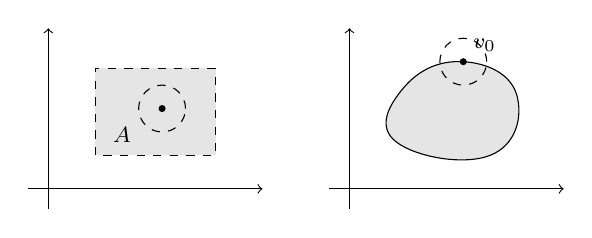
\begin{tikzpicture}[scale=0.85]
    % Primo grafico: punto interno
    \draw[->] (-0.3,0) -- (3.2,0);
    \draw[->] (0,-0.3) -- (0,2.4);
    \fill[gray!20] (0.7,0.5) rectangle (2.5,1.8);
    \draw[dashed] (0.7,0.5) rectangle (2.5,1.8);
    \fill (1.7,1.2) circle (1.5pt);
    \draw[dashed] (1.7,1.2) circle (0.35);
    \node at (1.1,0.8) {\footnotesize $A$};

    % Secondo grafico: punto non interno (sul bordo)
    \begin{scope}[xshift=4.5cm]
        \draw[->] (-0.3,0) -- (3.2,0);
        \draw[->] (0,-0.3) -- (0,2.4);
        \filldraw[fill=gray!20, draw=black] plot[smooth cycle, tension=0.8] coordinates {(0.7,0.7) (2.1,0.5) (2.5,1.4) (1.7,1.9) (0.8,1.5)};
        \fill (1.7,1.9) circle (1.5pt) node[above right] {\footnotesize $v_0$};
        \draw[dashed] (1.7,1.9) circle (0.35);
    \end{scope}
\end{tikzpicture}
\end{center}

Un punto $(x_0, y_0) \in \mathbb{R}^2$ si dice \underline{esterno} ad $A$ se
\[
\exists I_\delta(x_0, y_0) : I_\delta(x_0, y_0) \cap A = \emptyset
\]

\begin{itemize}
    \item $(x_0, y_0) \in \mathbb{R}^2$ si dice \underline{punto di frontiera} per $A$ se non è né interno né esterno ovvero $\forall I_\delta(x_0, y_0)$ si ha
    \[
    I_\delta(x_0, y_0) \cap A \neq \emptyset
    \]
    \[
    I_\delta(x_0, y_0) \setminus A \neq \emptyset
    \]
    L'ins. di pti di frontiera si indica con \underline{$\partial A$} e si chiama \underline{frontiera}.

    \item $(x_0, y_0) \in \mathbb{R}^2$ si dice \underline{isolato} se $\exists I_\delta(x_0, y_0)$:
    \[
    I_\delta(x_0, y_0) \cap A = \{ (x_0, y_0) \}
    \]
    \pencilnote{(i pti di front. non sono mai isolati)}

    \item Un ins. $A \subseteq \mathbb{R}^2, A \neq \emptyset$ si dice \underline{aperto} se tutti i suoi punti sono interni.

    \item $C \subseteq \mathbb{R}^2$ si dice \underline{chiuso} se $\mathbb{R}^2 \setminus C$ è aperto.
    \pencilnote{(gli aperti non devono contenere i propri ``contorni'')}
\end{itemize}

\begin{center}
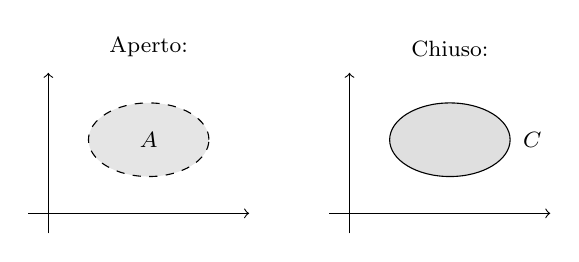
\begin{tikzpicture}[scale=0.85]
    % Aperto
    \node[above] at (1.5,2.2) {\footnotesize Aperto:};
    \draw[->] (-0.3,0) -- (3.0,0);
    \draw[->] (0,-0.3) -- (0,2.1);
    \fill[gray!20] (1.5,1.1) ellipse (0.9 and 0.55);
    \draw[dashed] (1.5,1.1) ellipse (0.9 and 0.55);
    \node at (1.5,1.1) {\footnotesize $A$};

    % Chiuso
    \begin{scope}[xshift=4.5cm]
        \node[above] at (1.5,2.2) {\footnotesize Chiuso:};
        \draw[->] (-0.3,0) -- (3.0,0);
        \draw[->] (0,-0.3) -- (0,2.1);
        \fill[gray!25] (1.5,1.1) ellipse (0.9 and 0.55);
        \draw (1.5,1.1) ellipse (0.9 and 0.55);
        \node[right] at (2.45,1.1) {\footnotesize $C$};
    \end{scope}
\end{tikzpicture}
\end{center}

\begin{itemize}
    \item Sia $A \subseteq \mathbb{R}^2, A \neq \emptyset$. $(x_0, y_0)$ si dice \underline{pto di acc.} per $A$ se $\forall I_\delta(x_0, y_0)$ risulta
    \[
    I_\delta(x_0, y_0) \cap A \setminus \{ (x_0, y_0) \} \neq \emptyset
    \]

    \item $A \subseteq \mathbb{R}^2, A \neq \emptyset$ si dice \underline{limitato} se $\exists I_R(v_0)$ tale che
    \[
    A \subset I_R(v_0)
    \]

    \item Un ins. $K \subseteq \mathbb{R}^2$ si ``dice'' \underline{compatto} se è chiuso e limitato \pencilnote{(in realtà è Heine-Borel)}.
\end{itemize}

\begin{center}
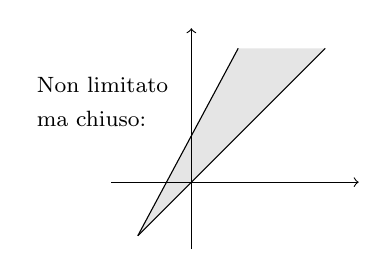
\begin{tikzpicture}[scale=0.85]
    \node[left, align=left] at (-0.2,1.2) {\footnotesize Non limitato \\ \footnotesize ma chiuso:};
    \fill[gray!20] (-0.8,-0.8) -- (2.0,2.0) -- (0.7,2.0) -- (-0.8,-0.8);
    \draw[->] (-1.2,0) -- (2.5,0);
    \draw[->] (0,-1.0) -- (0,2.3);
    \draw (-0.8,-0.8) -- (2.0,2.0);
    \draw (-0.8,-0.8) -- (0.7,2.0);
\end{tikzpicture}
\end{center}

\begin{note*}
$\mathring{A} =$ \underline{parte interna} di $A$: è il più grande aperto contenuto in $A$.

$\overline{A} =$ \underline{chiusura} di $A = A \cup \partial A$.
\end{note*}

\begin{example}
Dominio di $f(x, y)$:
\[
f(x, y) = \frac{\log(x - \vert y \vert) + \sqrt{3 - (x^2 + y^2)}}{\sqrt[4]{x^2 - y}}
\]
\[
E = \{ (x, y) \in \mathbb{R}^2 : \vert y \vert < x, \ x^2 + y^2 \le 3, \ x^2 > y \}
\]
\begin{center}
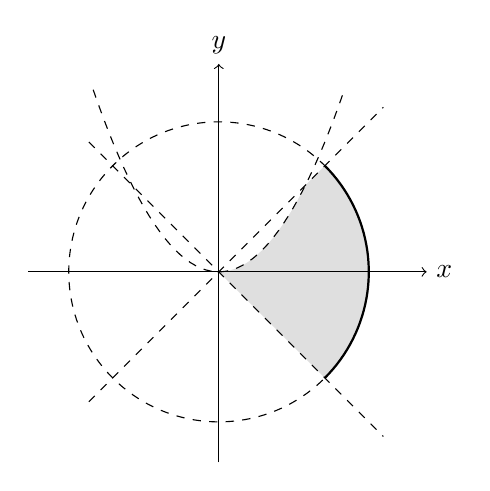
\begin{tikzpicture}[scale=1.1]
    % Regione E: -x < y < x, x^2 + y^2 <= 3, y < x^2
    \fill[gray!25] (0,0) -- plot[domain=0:1, samples=30] (\x, {\x*\x}) -- plot[domain=45:-45, samples=40] ({sqrt(3)*cos(\x)}, {sqrt(3)*sin(\x)}) -- cycle;
    % Assi
    \draw[->] (-2.2,0) -- (2.4,0) node[right] {$x$};
    \draw[->] (0,-2.2) -- (0,2.4) node[above] {$y$};
    % Circonferenza x^2 + y^2 = 3 (tratteggiata fuori, continua sul bordo di E)
    \draw[dashed] (0,0) circle ({sqrt(3)});
    \draw[thick] plot[domain=-45:45, samples=40] ({sqrt(3)*cos(\x)}, {sqrt(3)*sin(\x)});
    % Bisettrici y = x e y = -x
    \draw[dashed] (-1.5,-1.5) -- (1.9,1.9);
    \draw[dashed] (-1.5,1.5) -- (1.9,-1.9);
    % Parabola y = x^2
    \draw[dashed] plot[domain=-1.45:1.45, samples=50] (\x, {\x*\x});
\end{tikzpicture}
\end{center}
\end{example}

\subsection{Insiemi connessi, convessi e stellati}

\begin{definition}
Sia $A \subseteq \mathbb{R}^2$, $A \neq \emptyset$ e $A$ \underline{aperto}. $A$ si dice \underline{connesso} se ogni volta che $\exists A_1, A_2$ aperti:
\begin{enumerate}
    \item $A = A_1 \cup A_2$
    \item $A_1 \cap A_2 = \emptyset$
\end{enumerate}
allora deve accadere che $A_1 = \emptyset$, $A_2 = A$.
\end{definition}

\begin{center}
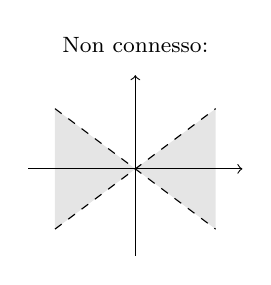
\begin{tikzpicture}[scale=0.85]
    \node[above] at (0,1.6) {\footnotesize Non connesso:};
    \fill[gray!20] (0,0) -- (1.2,0.9) -- (1.2,-0.9) -- cycle;
    \fill[gray!20] (0,0) -- (-1.2,0.9) -- (-1.2,-0.9) -- cycle;
    \draw[->] (-1.6,0) -- (1.6,0);
    \draw[->] (0,-1.3) -- (0,1.4);
    \draw[dashed] (-1.2,-0.9) -- (1.2,0.9);
    \draw[dashed] (-1.2,0.9) -- (1.2,-0.9);
\end{tikzpicture}
\end{center}

\begin{oss}
$A \subseteq \mathbb{R}^2, A \neq \emptyset$ è connesso se lo è $\mathring{A}$.
\end{oss}

\begin{definition}
$A \subseteq \mathbb{R}^2, A \neq \emptyset$ si dice \underline{convesso} se $\forall$ coppia di suoi punti $P, Q \in A$, il seg. che li cong. è contenuto in $A$.

È ovvio che $\text{conv.} \implies \text{conn.}$
\end{definition}

\begin{definition}
$A \subseteq \mathbb{R}^2$ si dice \underline{stellato} rispetto a $(x_0, y_0)$ se $\forall$ punto $P \in A$ il segmento che congiunge $P$ ad $(x_0, y_0)$ è contenuto in $A$. $(x_0, y_0)$ si dice \underline{centro della stella}.
\end{definition}

\begin{center}
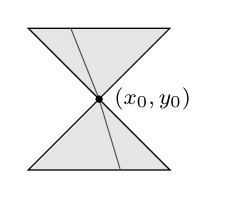
\begin{tikzpicture}[scale=0.9]
    \fill[gray!20] (-1,1) -- (1,1) -- (0,0) -- (1,-1) -- (-1,-1) -- (0,0) -- cycle;
    \draw (-1,1) -- (1,1) -- (-1,-1) -- (1,-1) -- cycle;
    \draw[gray!70!black] (0,0) -- (-0.4,1);
    \draw[gray!70!black] (0,0) -- (0.3,-1);
    \fill (0,0) circle (1.5pt) node[right=2pt] {\footnotesize $(x_0, y_0)$};
\end{tikzpicture}
\end{center}

\begin{definition}
$A \subseteq \mathbb{R}^2, A \neq \emptyset$, si dice \underline{connesso per poligonali} se $\forall P, Q$ di $A$ $\exists$ una spezzata che li congiunge e contenuta in $A$.
\end{definition}

\begin{oss}
Se $A$ è aperto $\implies$ connesso $=$ connesso per poligonali.

Se $A$ non è aperto $\implies$ connesso $\neq$ conn. per poligonali.
\end{oss}
